% !TeX spellcheck = cs_CZ
{\tikzset{external/prefix={tikz/FYZI/}}
 \tikzset{external/figure name/.add={ch22_}{}}
%=========================== Kapitola: Algebra =====================================================
\chapter{Algebra}\label{fyz:IchapXXII}
\minitoc
\section{Sčítání a násobení}\label{fyz:IchapXXIIsecI}
\section{Inverzní operace}\label{fyz:IchapXXIIsecII}
\section{Abstrakce a zobecnění}\label{fyz:IchapXXIIsecIII}
\section{Aproximace iracionálních čísel}\label{fyz:IchapXXIIsecIV}
\section{Komplexní čísla}\label{fyz:IchapXXIIsecV}
\section{Imaginární exponenty}\label{fyz:IchapXXIIsecVI}
\section{Příklady a cvičení}\label{fyz:IchapXXIIsecVIII}

  \begin{figure}[ht!] %\ref{fyz_fig413}
    \centering
    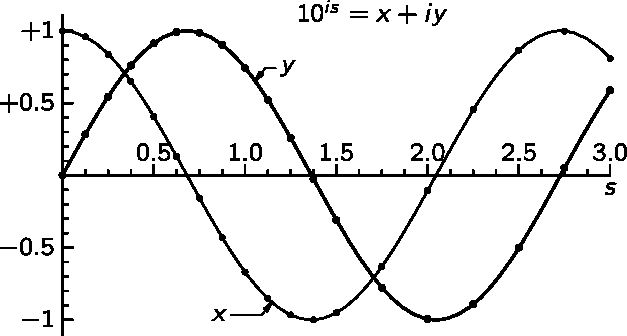
\includegraphics[width=0.3\linewidth]{fyz_fig413.pdf}
    \caption{
             (\cite[s.~306]{Feynman01})}
    \label{fyz_fig413}
  \end{figure}

  \begin{figure}[ht!] %\ref{fyz_fig414}
    \centering
    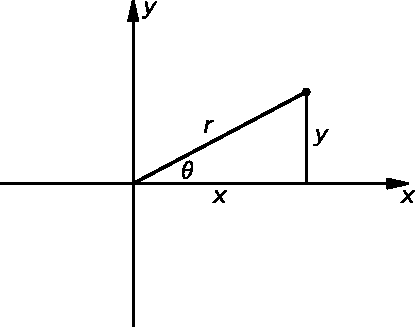
\includegraphics[width=0.3\linewidth]{fyz_fig414.pdf}
    \caption{\(x + y = re^i\)
             (\cite[s.~306]{Feynman01})}
    \label{fyz_fig414}
  \end{figure}
  
} %tikzset
%---------------------------------------------------------------------------------------------------
\printbibliography[title={Seznam literatury}, heading=subbibliography]
\addcontentsline{toc}{section}{Seznam literatury}